\documentclass[11pt, oneside]{article}   	% use "amsart" instead of "article" for AMSLaTeX format
\usepackage{geometry}                		% See geometry.pdf to learn the layout options. There are lots.
\geometry{a4paper}                   		% ... or a4paper or a5paper or ... 
%\geometry{landscape}                		% Activate for for rotated page geometry
%\usepackage[parfill]{parskip}    		% Activate to begin paragraphs with an empty line rather than an indent
\usepackage{graphicx}				% Use pdf, png, jpg, or eps§ with pdflatex; use eps in DVI mode
\usepackage{array}							% TeX will automatically convert eps --> pdf in pdflatex		
\usepackage{amssymb}
\usepackage{cite}

\title{Requirement Engineering Process in AMIDST}
\author{The handsome AMIDST guys et. al.}
\date{Latest version, \today}							% Activate to display a given date or no date

\begin{document}
\maketitle
%
%\begin{abstract}
%\end{abstract}
%
\section{Introduction}

Even though the field of requirement engineering RE is mature and requirement engineering on very small software projects (less than 10 developers) are seen as quite immature as stated in \cite{Qui10}. In 2007, a study of seven very small software enterprises VSSE in Canada was conducted \cite{Ara07}..  The preliminary result was that 1) RE practices in successful VSSE are diverse and work well in organisations where they are applied, 2) all the companies that where studied had a strong cultural cohesion, 3) experienced persons where in charge of RE process and 4) requirement errors in these companies where rarely catastrophic.  Contrastingly, in 2011, a study of 24 experienced project managers from 24 different small software companies in Chile came to different conclusions \cite{Qui10}.  The study involved a survey of 48 questions and attending an hour long focal group for discussions.  The findings were that 1) project specifications were usually met, but the clients usually finds the solution unsatisfactory, 2) communication issues with the clients cause incomplete specifications, 3) scope creep is common 4) the RE process is often ad-hoc, 5) loss of requirements are common, 6) in cases of uncertainty, developers often finds solutions without contracting the clients and 7) VSSE are aware of RE practices but are not sure how to apply them.  Based on these two studies, it is clear that in practice RE processes are conducted very differently and experiences vary much.  Consequently, practical experiences do not point in a unified way to a common method for RE process on small projects.

In the literature, several ready-to-use approaches for RE on small projects are attempted.  In 2004, Nikula presented a basic RE model as part of his phd thesis \cite{Nik04}, but based on an argumentation in \cite{Qui10}, this method may not be suitable for VSSE projects, because the method is based on results from a study that involved mostly larger companies \cite{Nik00}.   Dorr et. al. presented a set of 36 RE practices for RE improvement for small software projects \cite{Dor08}.  However, in this research the six companies that was considered had between 20 and 200 employees, meaning that this research was biased towards medium sized projects rather than VSSE. It is also worth mentioning that a large portion of modern software companies follows Agile methods for software development \cite{Din10}.  
Paper \cite{Kav11} outlines how to incorporate requirement gathering in small Agile projects.  However, in the Agile methodology, requirement engineering is seen as an ongoing process involving a product owner that continuously is renegotiating the requirements.  Due to the project management process in EU, the AMIDST project is limited from following such a process. 

Based on the lack of clarity in practice and consensus in literature on a common RE process for small projects, we decided to identify the characteristics of our project and motivate our choices of RE process from this.  For instance, the AMIDST project is characterized by the fact that there is a description of work that is agreed upon upfront.  The 
AMIDST RE process must comply with the STREP proposal FP7-ICT-2013-11, and in more particular the software must comply with all deliveries in work package 1 to 8. 
%task 2.3 in work package 2, tasks; 3.3, 3.4, 3.5, 3,6 and 3.7 in work package 3, tasks; 4.1, 4,2 4,3 and 4.4 in work package 4 and tasks; 5.1, 5,3, 5,4 and 5,6 in work package 5.
Another important characteristic, is that there is a huge widespread of stakeholders in the project and that the software is required to interface with three different softwares from three different companies.  Because of this, a clear focus has been put on functional requirements, which are the requirements that are most transparent to the user.  As will be discussed more later, a use case driven approach xx is taken to achieve this.

The report is outlined as follows.  In section \ref{sec:stateOfArt}, the basic principles of in modern requirement engineering are briefly outlined.  Section \ref{sec:AmidstRequirementProcess} starts by describing the main characteristics of the AMIDST project, before the requirement engineering process is outlined.  In section \ref{sec:realization}, we have described the realisation of the process so far, before the report is concluded in section \ref{sec:conclusion}.


\section{Basic principles in requirement engineering}
\label{sec:stateOfArt}

In practice, the requirement engineering process ends with a document containing a list with requirements, which are in the form of what a software must do or comply with.  There is agreement that a definition of a requirement is related to \emph{what} a system can do and not \emph{how} it is done.  

To date there is no common definition of requirement engineering.  Some definitions focus on elicitation of requirements and therefore the interaction with the user, while others focus on the documentation or the specification.  A definition that takes both focuses into account is the IEEE standard given in \cite{Iee90}:

\emph{
\begin{enumerate}
\item The process of studying user needs to arrive at a definition of system, hardware or software requirements.
\item The process of studying and refining system, hardware or software requirements.
\end{enumerate}
}

In the context of understanding the requirement engineering process, it is worth spending some space defining the requirement itself.  A definition of a requirement is given in IEEE standard \cite{Iee90}: 
\emph{
\begin{enumerate}
\item A condition or capability needed by a user to solve a problem or achieve an objective. 
\item A condition or capability that must be met or possessed by a system or system component to satisfy a contract, standard, specification or other formally imposed document. 
\item A documented representation of a condition or capability as in 1 or 2.
\end{enumerate}
}

This definition has a clear focus on the user, the system/system component and also which contract, standard or specification is needed to be met. 

\subsection{Product lifecycle}

In order for a requirement to be useful for the software engineers, they are often associated with steps in a product life cycle as for instance described in \cite{Eig09}.  In this reference the overall life cycle is divided into three phases; design phase, operation phase and disposal phase, see figure \ref{REprocess2}.

\begin{figure}
\centering
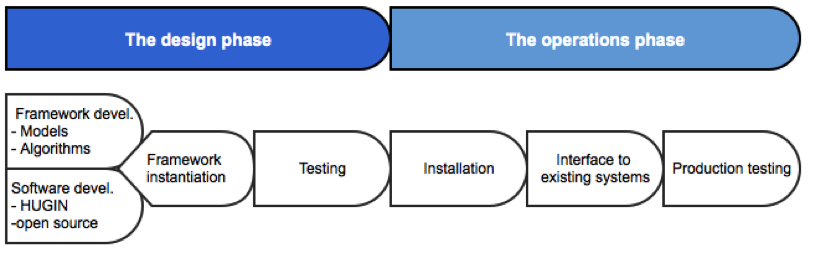
\includegraphics [keepaspectratio,width = 14cm] {REprocess2}
\caption{The table show key steps in the design and operation stages. Notice that each requirement can only be member of one step.  The third step is removed (TODO add to figure )}
\label{REprocess2}
\end{figure}

The design stage contains general functionality requirements for the system, i.e. what the system should do and support.  In figure \ref{REprocess2}, we detail key steps inside this phase. The first step consists of the design of the general framework (models and algorithms) as well as the design and development of the software tools. In a second step, the general framework and software is instantiated for each specific use case. Finally, initial tests of the use case instantiated framework are conducted.  At the design phase, possible design requirements could e.g. address
\begin{itemize}
 \item the scope of the model
 \item the interpretability of the learned models
 \item the extent and type of domain knowledge that can be integrated into the models
 \item documentation
\end{itemize}

The requirements for the operation phase concern the functionality of the deployed system. In figure \ref{REprocess2}, we decompose this phase into three stages: installation, interface to existing systems, and production testing. The requirements for this phase could e.g. address
\begin{itemize}
 \item hardware constraints
 \item interfaces to existing software or data base systems
 \item inference functionality, i.e., what queries the system should be able to answer
\end{itemize}


\subsection{Activities involved in requirement engineering}

The activities involved in requirements engineering vary widely, depending on the type of system being developed and the specific practices of the organization(s) involved  \cite{Som11}.  These may include:
\begin{itemize}
\item Requirements inception or requirements elicitation 
\item Requirements identification - identifying new requirements
\item Requirements analysis and negotiation - checking requirements and resolving stakeholder conflicts
\item Requirements specification (Software Requirements Specification) - documenting the requirements in a requirements document
\item System moddeling - deriving models of the system, often using a notation such as the Unified Modeling Language
\item Requirements validation - checking that the documented requirements and models are consistent and meet stakeholder needs
\item Requirements management - managing changes to the requirements as the system is developed and put into use
\end{itemize}

These activities are sometimes presented as chronological stages although, in practice, there is considerable interleaving between them.  

\subsection{Use case driven requirement engineering}

It has always been a challenge for the software industry to communicate functionality to the users of a software. Moreover, software engineers are often frustrated, because users often do not know what they want. They only have an idea of what they want.  To improve this communication, the use-case driven approach was developed in the nineties, first published by  \cite{Jac92}.  More on use cases can for instance be found in \cite{Poh10} and \cite{Coc01}.  A use case focuses only on the interaction between a user and the system and requirements are always associated with a use case. This means that the user is requested to only focus on what he/she wants.  This is an advantage, compared to the traditional way where requirements are listed in relation to components and subcomponents in the software.  The traditional way often lead to a complexity that a user do not understand.  Also, it is more common with requirement duplicates in the traditional approach.

A use case is a list of steps, typically defining interactions between an actor and a system, to achieve a goal. The actor can be a human or an external system.  An overview on how to write effective use cases is given in \cite{Coc01}, where several templates are given. The use case providers are asked to provide the use cases in natural language and for each use case the following questions are central:

\begin{enumerate}
\item Who are the actors involved in the use case? An actor is either a person or an entity that interacts with the software.  
\item What is the main event that initiates the use case? This could e.g. be an external business event or a system event that causes the use case to begin.  It could also be the initial step in a normal work flow. 
\item What are the main user actions and system responses that will take place during the normal execution of the use case?. This dialog sequence will ultimately lead to accomplishing the goal that is implied by the use case name and description.
\item How can we evaluate the success of the use case?
\end{enumerate}
 
It is also common to group the users, or human actors, within an organisation into a small set of user groups. The users within each user group need to have similar roles within their organisation and their set of competences are expected to be similar. 

To understand the use case driven approach to requirement engineering better it is useful to distinguish between functional and non functional requirements.  Functional requirements are those requirements that are directly related to the interaction between the user and the system.  The non functional requirements are more hidden for the user are related to the global overall success.  For instance scalability, traceability and testability.  When use cases are provided and functional requirements are identified, it is the requirement engineers role to identify, document and communicate these non functional requirements as well.  The use case driven approach to requirement engineering focuses on revealing the functional requirements together with the users.  This improves the communication between the users and the developers, because the focus is on what the users wants and less on how it can be done.

\section{The AMIDST requirements engineering process}
\label{sec:AmidstRequirementProcess}

In this section we describe the AMIDST engineering process by first describing some characteristics with this particular project.  Prior to project start, the importance of requirement engineering was well acknowledged by the partners in the project.  This is evident from the fact that 23 out of 310 person months were assigned to conduct the requirement analysis.  We have chosen to summarise the characteristics in the next subsections, which makes it is easier to refer to them later in this report.

\subsection{Characteristics of the AMIDST project}
\label{sec:characteristics}

\subsubsection{Characteristics one: Many partners on different locations}
\label{sec:characteristic1}
The project is a consortium of 7 partners, 4 industrial and 3 universities, which are situated in 4 different countries.  Many partners means many stakeholders to the project, which again means that it is more challenging to agree on requirements.  Moreover, when the partners are located in different countries, it is more costly to meet in person.

\subsubsection{Characteristics two: Transference of domain knowledge from industrial partners}
\label{sec:characteristic2}
The software is expected to be compatible with three different systems in three different domains, with three different companies.  In the AMIDST project, we are expecting to solve difficult problems in the industrial domains that have not been solved before.  The developers of the software are mainly from the academic partners.  It is therefore essential that the academic partners gain enough knowledge about the industrial domains and also the systems that the AMIDST software is going to interact with. 

\subsubsection{Characteristics three: Transference of domain knowledge from academic partners}
\label{sec:characteristic3}
The software itself is based on probabilistic graphical models.  Often, the discussions between the academic and the industrial participants only involves discussing causal relations between variables in a Bayesian network.  This is usually comprehendible for most users of a system.  However, discussions often need to go deeper than this and this leads to more theoretical reflections which are difficult for many industrial participants. 

\subsubsection{Characteristics four: Targets are highly innovational}
\label{sec:characteristic4}
Defining a requirement is linked with the perception of which design pattern to follow \cite{Ral13}.  A design pattern is chosen by the software developer and is basically the path to meet the requirement.  As explained in \cite{Ral13}, when there is a high degree of unclarity of which design design pattern to follow, this ambiguity is transferred to the definition of the requirement as well.  The goal of the AMIDST software is to reach targets that are highly innovational, meaning that it is particularly difficult to define requirements that are clear and unambiguous.

\subsubsection{Characteristics five: Compliance with EU application}
\label{sec:characteristic5}
The requirement engineering document and the requirement engineering process itself must be in compliance
with the approved application to the seventh EU programme. It is not enough that the software fulfil the need of the users, but it must also comply with the tasks that are promised in this project. 

\subsection{The AMIDST requirements engineering process}
\label{sec:reprocess}

The overall requirement engineering process is carried out in an iterative fashion that is expected to involve a high level of cooperation and interaction between the partners in order to meet all characteristics in subsection \label{sec:characteristics}.  A use case driven approach, which has a focus on functional requirements, is chosen to meet challenge two and three in particular.  

In figure \ref{REprocess1}, an illustration of the requirement engineering process for AMIDST is given, which is inspired by \cite{Ebe10}.  In general the process contain five phases, which are discussed below.
\begin{enumerate}
\item Preparation I.  This phase starts at the same time as Work Package 1 and ends when the initial template, attachment X1, for the requirement engineering document is finished.  In this template, the requirement engineering process is outlined including definitions of use cases, user groups and how to link requirements with stages in development process.  In order to meet challenge two, the use case providers are asked to provide a detailed description of the system context that the AMIDST software is expected to run in, identify user groups, describe use cases and requirements.  In order to meet characteristics three, the requirements are linked with references to stages in the development cycle.  In the AMIDST project lifcycle we only considered the two first phases and figure \ref{REprocess2}.
\item Elicitation. The distribution of the above mentioned template marks the initialisation of this phase.  Its aim is to get an initial high-level description of the different use cases and their requirements. This information are specified by the use case providers in collaboration with the academic partners to meet characteristic two, three and five.  Once the use case providers return the present document with the requested information, feedback and informal meetings are expected to clarify and refine the information provided.  At the end of the elicitation phase, the aim is to have a first coherent description of the requirements for each use case provider.
 \item Prioritization. In this phase the use case providers completes an extended version of the document template used in the previous phase. This template is used to link each of the requirements to the relevant work packages and tasks in the AMIDST project to meet characteristics five. Moreover, the template allows the use case providers to provide a more fine grained prioritization of the relevant requirements for the AMIDST framework.  Specifically, the use case providers are asked to rate each requirement in terms of must, should and could and also rate how important it is to them.  
\item Validation. In this phase, the requirements from all use-case providers are collected to get the \emph{big picture}.  This involves a discussion to what extent the requirements can be accommodated. Revisions and negotiations of the detailed requirements are therefore expected.  In this step it is of key importance to ensure that characteristics five is met.
 \item Evaluation and Testing. In this phase, the focus is on the elicitation of the evaluation and testing procedures in the AMIDST project. This phase starts with the distribution of a new document template, where the aim is to obtain a high level description of the evaluation and testing methods that is necessary to measure the performance of the AMIDST framework.
\end{enumerate}

\begin{figure}
\centering
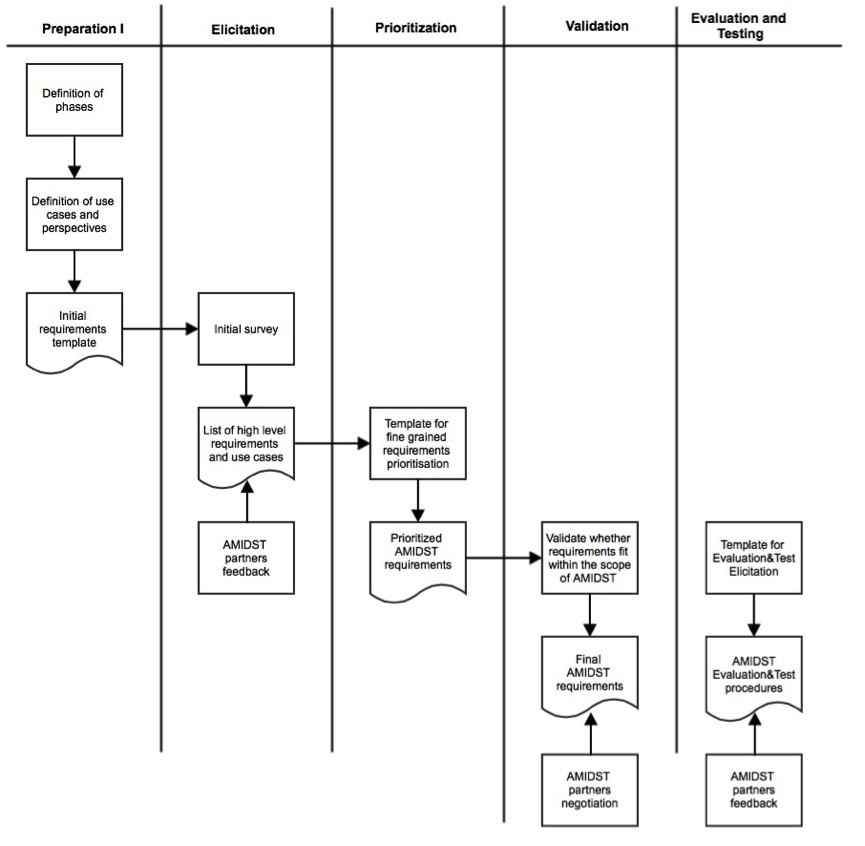
\includegraphics [keepaspectratio,width = 14cm] {REprocess1}
\caption{Description of the five phases in the requirement engineering process in AMIDST.}
\label{REprocess1}
\end{figure}

\section{Realization of the requirements engineering process}
\label{sec:realization}

It is appropriate to make a few comments related to characteristics two in table \ref{tab:characteristic} and also the need for massive knowledge transfer in the project.  No constraints on the form of the meetings are set.  Communication is done through meetings, video calls, telephone, email and document transferral.  The participants in the meetings could range from a large group to only a few people.  The reason for the \emph{no constraint policy} is to encourage as much knowledge transfer as possible.  The formal parts are taken into account in the requirement engineering documents that will be delivered at the end of the requirement engineering process. 


\section{Conclusion, observations and reflections}
\label{sec:conclusion}

This part of the report is written in month six when most of the process is conducted.  This section contains a few points on what experiences we have gained in the project so far

Some important experiences in this project have been:

\begin{enumerate}
\item Everyone involved has had a learning experience on many levels.  The industrial partners have learned about probabilistic graphical models, while the academic partners have learned about the industrial domains.  Most participants have increased their knowledge on how to conduct a requirement analysis. 
\item There has only been one meeting where all stakeholders have met, which was the kickoff meeting in Denmark in month three.  Most communication has been done through Skype and email, but also a few face to face meetings have taken place. Most of the communications have been related to clarifications in terms of filling out the template X1.
\item There have been adjustments of the template X1 as the process has proceeded.  Examples of this is adding fields to the requirements so they could be linked to concrete tasks in the AMIDST project or adding columns for rating the importance of a requirement.
\end{enumerate}










\bibliographystyle{splncs}
\bibliography{re}


\end{document}  